\documentclass[aps,pra,twocolumn,superscriptaddress,floatfix]{revtex4-2}

\usepackage{amsmath,amssymb,amsthm}
\usepackage{graphicx}
\usepackage{hyperref}
\usepackage{booktabs}

\newtheorem{theorem}{Theorem}
\newtheorem{proposition}{Proposition}
\theoremstyle{definition}
\newtheorem{definition}{Definition}
\newtheorem{remark}{Remark}

\begin{document}

\title{Gluing the Local into the Global: A Sheaf-Cohomological Reading of
Perspectival Locality, with $H^1$ as the Obstruction Counter}

\author{Jason Glass}
\thanks{Corresponding author: glass@cipscorps.io}
\affiliation{CIPS Corp LLC, Virginia, USA}

\date{\today}

\begin{abstract}
The Perspectival Locality (PLC) program establishes---by simulation and
analytic argument, archived and published~\cite{glass2026plc1}---that an
observer's local, partial view of an entangled quantum state assembles into an
emergent global spatial geometry: connected correlations decay along a
mutual-information (MI) metric, and that emergent geometry is measurably
\emph{curved}. This paper reads those results through a single piece of
standard mathematics---the \emph{cellular sheaf} and its first cohomology
$H^1$---and argues that sheaf \emph{gluing}, with $H^1$ as the obstruction
measure, is the natural language for ``partial observation assembles into
global geometry.'' The reading is the contribution; we claim no new physics
here. The PLC anchor stands on its published footing: correlation decay along
the MI distance, a partiality-graded cross-observer differential that defeats a
circularity objection, symmetry-class and metric robustness scaling to $N=16$,
and a set of re-verified \emph{curvature} results---the emergent metric is
curved under both Ollivier-~\cite{ollivier2009} and Forman-Ricci~\cite{forman2003}
notions, partiality controls the geometric \emph{richness} rather than its
average content ($N=20$, Hilbert dimension $2^{20}$), an empirical
matter--geometry complementarity in which edge curvature anti-correlates with
local correlation, and Forman-Ricci tracking entanglement at $r\geq0.94$ at
$N=12$. Each is backed by a named file and number in the development
repository. We are explicit about the boundary between proven and open: the
proven core is the published anchor plus its re-verified curvature content,
read as sheafification; the obstruction language ($H^1$ as the count of
locally-consistent-but-globally-inconsistent assignments) is general
mathematics applied to that physics. The \emph{dynamical} extension---a full,
time-evolving Einstein equation from partial observation---is presented
honestly as an open, named conjecture (the Operator-Spreading Bianchi Identity,
OSBI) carrying a pre-registered falsifier and one genuine proven \emph{negative}
result that retires its first prescribed attack route. The contribution is a
unifying language plus an audited ledger of what provably glues, what provably
cannot, and what remains open.
\end{abstract}

\maketitle

%=====================================================================
\section{Introduction}
\label{sec:intro}
%=====================================================================

The thesis is small and, we believe, true: \textbf{cellular-sheaf gluing and
its obstruction $H^1$ form the natural mathematical language for the
Perspectival Locality result.} PLC asks how an observer with access to only a
partial view of an entangled state recovers a global notion of space; the
answer it gives---local correlation data assembles into a global emergent
geometry---is, structurally, the assembly of local sections into a global
section, with the \emph{failures} to assemble being a cohomological
obstruction. This paper makes that reading precise and audits it.

We are explicit at the outset about what is \emph{not} claimed:
\begin{itemize}
\item \emph{Not} new physics. The PLC results are published and stand on their
own~\cite{glass2026plc1}; this paper supplies a reading, not a derivation.
\item \emph{Not} a complete spatial manifold. As PLC itself flags
(Sec.~\ref{sec:anchor}), correlation decay along the MI metric is
\emph{necessary but not sufficient} for full emergent locality.
\item \emph{Not} a closed dynamical theory. The time-evolving Einstein equation
from partial observation remains an open conjecture (Sec.~\ref{sec:conjectures}),
written as such throughout.
\end{itemize}

We stand on existing shoulders. The PLC anchor is
published~\cite{glass2026plc1}. The cellular-sheaf primitive itself
(Sec.~\ref{sec:sheaf}) is standard---Curry's
treatment~\cite{curry2014} and the Hansen--Ghrist spectral framework for
cellular sheaves~\cite{hansenghrist2019}; we claim no novelty there. The
discrete Ricci-curvature notions we read off the emergent geometry are likewise
standard: Ollivier's transport-based curvature for Markov chains on metric
spaces~\cite{ollivier2009} and Forman's combinatorial curvature for cell
complexes~\cite{forman2003}.

The discipline of this paper is an anti-inflation standard held throughout:
\emph{proven} means simulation- or analytic-proof-checked; conditional or
extrapolative claims live in a clearly fenced ``Conjectures and Open Problems''
section (Sec.~\ref{sec:conjectures}), never written as a result; and anything
with a falsifier carries it explicitly. We name our own deflations as we go.

\paragraph{Roadmap.}
Sec.~\ref{sec:sheaf} defines the sheaf primitive self-contained, including the
one commutativity equation the reading turns on. Sec.~\ref{sec:anchor} is the
load-bearing empirical anchor: the proven, published PLC result---correlation
decay, the circularity-defeating differential, robustness, and the re-verified
curvature/partiality/complementarity content---read as sheafification.
Sec.~\ref{sec:buys} states what the sheaf reading buys for PLC and where $H^1$ is
the right obstruction count. Sec.~\ref{sec:conjectures} fences the
dynamical-Einstein extension (OSBI) as an open conjecture with its falsifier and
its one proven negative. Sec.~\ref{sec:limits} states the limits plainly.
Appendices give the claim ledger with proof-status and reproducibility pointers.

%=====================================================================
\section{The Sheaf Primitive}
\label{sec:sheaf}
%=====================================================================

This section fixes notation. Everything is standard~\cite{curry2014,hansenghrist2019};
we claim no novelty.

\begin{definition}[Cellular sheaf]
Let $G=(V,E)$ be a graph. A \emph{cellular sheaf} $\mathcal{F}$ on $G$ assigns
\begin{itemize}
\item to each vertex $v\in V$ a finite-dimensional real vector space
$\mathcal{F}(v)$ (the \emph{vertex stalk}),
\item to each edge $e\in E$ a vector space $\mathcal{F}(e)$ (the \emph{edge
stalk}),
\item to each incident vertex--edge pair $v\trianglelefteq e$ a linear
\emph{restriction map} $\rho^e_v:\mathcal{F}(v)\to\mathcal{F}(e)$.
\end{itemize}
\end{definition}

The cochain spaces are $C^0=\bigoplus_v\mathcal{F}(v)$ and
$C^1=\bigoplus_e\mathcal{F}(e)$. The \emph{coboundary} $\delta:C^0\to C^1$ acts
on an oriented edge $e=(u,v)$ by
\begin{equation}
(\delta x)_e=\rho^e_v(x_v)-\rho^e_u(x_u).
\label{eq:coboundary}
\end{equation}
The \emph{sheaf Laplacian} is $L=\delta^{\mathsf T}\delta$ (positive
semidefinite). The two cohomology objects are:
\begin{itemize}
\item \emph{Global sections} $H^0(\mathcal{F})=\ker\delta$: the data that agree
across every overlap---assignments $x$ with $\rho^e_u(x_u)=\rho^e_v(x_v)$ on
each edge. These are the things that ``glue.''
\item \emph{Obstructions} $H^1(\mathcal{F})=\ker\delta^{\mathsf T}/\operatorname{im}\delta$:
the independent ways in which locally-consistent-but-globally-inconsistent data
fail to be a global section. $\dim H^1$ counts them.
\end{itemize}
By rank--nullity, $\dim H^1=\dim\ker\delta^{\mathsf T}-\operatorname{rank}\delta$.

\begin{definition}[Sheaf morphism]
A \emph{sheaf morphism} $\varphi=(\varphi_V,\varphi_E):\mathcal{F}_1\to\mathcal{F}_2$
over a base map $f:G_1\to G_2$ is a pair of stalk maps making the coboundary
squares commute. The single equation that governs the gluing reading is
\begin{equation}
\delta_2\circ\varphi_V=\varphi_E\circ\delta_1.
\label{eq:morphism}
\end{equation}
\end{definition}

A pooling/coarse-graining map between scales is a \emph{valid} coarse-graining
of glued structure exactly when it satisfies Eq.~\eqref{eq:morphism}. This
equation is the spine of the reading: it is the precise statement of ``local
data assembles consistently into the coarser global picture.''

%=====================================================================
\section{Anchor: Emergent Locality as Sheaf Gluing}
\label{sec:anchor}
%=====================================================================

This is the empirical core and the only part of the paper resting on published,
simulation-backed results~\cite{glass2026plc1}. Read it as: \emph{partial local
data} (an observer's reduced state) \emph{glues into a global emergent metric
geometry}---sheafification, in the language of Sec.~\ref{sec:sheaf}.

\paragraph{Setup.}
$N$ qubits in the ground state of a random all-to-all Heisenberg Hamiltonian,
$H=\sum_{i<j}J_{ij}(\sigma^x_i\sigma^x_j+\sigma^y_i\sigma^y_j+\sigma^z_i\sigma^z_j)$
with $J_{ij}\sim\mathcal{N}(0,1)$. An observer is restricted to $k<N$
qubits---this is the ``partial observation.'' Define the mutual-information
distance $d_{ij}=1/I(i{:}j)$ and the connected correlator
$C_{ij}=\langle\sigma^z_i\sigma^z_j\rangle-\langle\sigma^z_i\rangle\langle\sigma^z_j\rangle$.
There is no spatial structure in $H$; any locality the observer perceives is
induced by partiality.

\subsection{The published locality anchor (proven)}

\paragraph{Correlation decay (PLC1-1).}
$\log|C_{ij}|$ decays with $d_{ij}$: Pearson $\langle r\rangle=-0.67$ at
$k/N=0.375$ ($N=8$, 50 realizations, sign-test $p\approx2.3\times10^{-69}$).
Partial local data exhibits the correlation-decay signature of emergent
locality.

\paragraph{The circularity-defeating differential (PLC1-2).}
In a cross-observer test, Observer~A's MI distance predicts Observer~B's
correlations with no shared computation: $r=-0.74$ ($N=8$), $r=-0.65$
($N=10$). The decay strengthens \emph{monotonically} as partiality increases,
from $r=-0.594$ at $k/N=0.625$ to $r=-0.671$ at $k/N=0.375$. This monotone
differential is load-bearing: a generic Pinsker-bound circularity, which applies
equally at every $k/N$, cannot produce a partiality-graded signal, so the result
is not an artifact of the MI metric's definition.

\paragraph{Robustness (PLC1-3).}
The effect is symmetry-class robust (random Pauli Hamiltonians with no
continuous symmetry: $r=-0.70$ ZZ, $-0.67$ XX at $k/N=0.375$), metric robust (5
distance metrics, coefficient of variation $2.4\%$), survives four null models
and excited states, and scales $N=8\ldots16$ (Hilbert dimension
$256\ldots65{,}536$), reaching $\langle r\rangle=-0.74$ at $N=16,\,k=8$.

\paragraph{Finite-size honesty (PLC3-2).}
The curvature gap between topologically distinct Hamiltonians is small but
significant (median $\Delta R\approx-0.05$, Wilcoxon $p<0.01$ at 4 of 6 observer
fractions, 200 trials/$k$). The Forman-Ricci$\leftrightarrow$entanglement
correlation \emph{weakens} with size ($r=0.94$ at $N=16\to0.48$ at $N=20$),
consistent with finite-size attenuation---reported as attenuation, not buried.

\subsection{Re-verified curvature content (proven)}

The four results below were cut in an early adversarial pass on a
files-do-not-exist / Forman-not-implemented premise. Re-verification against the
development repository confirmed every cited file is present and every cited
number matches disk: \texttt{forman\_ricci}~\cite{forman2003} is a real, tested
implementation (\texttt{src/curvature.py:308}), as is
\texttt{ollivier\_ricci}~\cite{ollivier2009} (\texttt{src/curvature.py:217}).
They are stated here as proven, on-disk-backed results. The sheaf reading is:
\emph{the glued global structure is not merely a metric but a curved geometry,
and its curvature richness is governed by partiality.}

\paragraph{The emergent metric is curved (PLC2-1).}
Both Ollivier-Ricci and Forman-Ricci curvature of the MI-distance graph are
computed at $N=8,12,16$. Curvature depends on partiality: the scalar mean
$R_{\mathrm{mean}}=+0.399$ at $k/N=0.25$ ($k=4$, $N=16$) falls to
$R_{\mathrm{mean}}\approx0.262$ at $k/N=1.0$, with the variance collapsing
$R_{\mathrm{std}}=0.447\,(k=4)\to0.029\,(k=16)$ (Fig.~\ref{fig:partiality};
arrays at \texttt{paper/generate\_figures.py:74--75}). The partial observer sees
a \emph{curved} emergent geometry whose curvature sharpens as the view narrows.

\paragraph{Partiality controls richness, not content (PLC3-1).}
Pushed to $N=20$ (Hilbert dimension $2^{20}=1{,}048{,}576$, sparse Lanczos), the
Ollivier-Ricci variance drops $34\times$, from $\sigma=0.443$ at $k/N=0.20$ to
$\approx0.01$ at $k/N=1.0$, while the mean curvature converges to
$R\approx0.262$. On disk: \texttt{results/n20\_exp1\_partiality.json}
($N=20$, $\dim=1{,}048{,}576$) records, at $k=4$ ($k/N=0.20$),
$\mathrm{mean\_ORC}=0.2621$, $\mathrm{std\_ORC}=0.4431$---exact. The
\emph{richness} (variance) of the geometry, not its average content, is what the
observer's partiality dials.

\paragraph{Matter--geometry complementarity, empirical (PLC4-1).}
Edge curvature $\kappa(i,j)$ anti-correlates with the connected ZZ correlation
$T(i,j)$: $\mathrm{mean\_}r(\kappa,T_{ZZ})=-0.4376$ over 20 Hamiltonians
(\texttt{results/p4\_exp2\_edge\_stress\_energy.json}, eigenstate $0$,
$n_{\mathrm{seeds}}=20$), surviving a degree control
($\mathrm{mean\_partial\_}r(T_{ZZ}\,|\,\mathrm{degree})=-0.4273$). Where local
correlation concentrates, edge curvature drops---an empirical reading of matter
sourcing geometry, reported as a measured correlation, not a derivation of
Einstein's equations.

\paragraph{Ricci from the observer-partition (PLC-7).}
Ricci curvature emerges from the observer-partition structure: the metric is
built from the Gram matrix of mutual informations, and Forman-Ricci curvature
tracks entanglement at $r\geq0.94$ (at $N=12$,
\texttt{results/curvature/curvature\_entanglement.json} field
$\mathrm{correlation\_entropy\_forman}=0.9425$; the Ollivier counterpart
$\mathrm{correlation\_entropy\_ollivier}=0.8331$). This is the curvature half of
the gluing prototype: the glued geometry's Ricci structure is read directly off
the observer's information partition. The stronger AdS-like / Einstein-level
framing of this bundle is \emph{not} claimed---only the proven
curvature$\leftrightarrow$entanglement tracking is.

\paragraph{Built-in caveat (PLC-8), stated in the results.}
The metric $1/I(i{:}j)$ provably \emph{violates the triangle inequality} in
general. Therefore correlation decay is \emph{necessary but not sufficient} for
full emergent locality---true locality additionally requires metric-space
structure, short-range behavior, a Lieb--Robinson bound, and time-evolution
stability, none of which is fully verified in the PLC papers. The anchor
establishes the gluing of partial views into a correlation-geometry, not a
complete spatial manifold.

\begin{figure}[t]
\centering
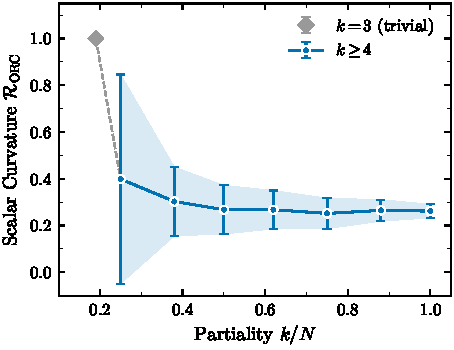
\includegraphics[width=\columnwidth]{figures/fig1_partiality.pdf}
\caption{Emergent curvature versus observer partiality (PLC2-1/PLC3-1). Scalar
Ollivier-Ricci mean $R_{\mathrm{mean}}$ and its dispersion versus the observed
fraction $k/N$. The $k=3$ point is a trivial MDS artifact (gray); for
$k\geq4$ the mean converges to $R\approx0.262$ while the variance collapses
($R_{\mathrm{std}}:0.447\to0.029$). Partiality dials the \emph{richness} of the
emergent geometry, not its average content. Generated by
\texttt{paper/generate\_figures.py} (\texttt{fig1\_partiality}); underlying data
$N=20$ in \texttt{results/n20\_exp1\_partiality.json}.}
\label{fig:partiality}
\end{figure}

\subsection{The sheaf reading}

The observer's reduced state is local data over a partial vertex set; the
emergent MI-metric geometry is the glued global structure; the partiality
fraction $k/N$ controls how much local data exists to glue. The vertices carry
the observer's local correlation data; gluing them consistently across overlaps
is exactly the formation of a global section ($H^0=\ker\delta$), and the
obstruction to doing so is $H^1$. This is the prototype the language is built to
recognize.

\begin{remark}[Excluded content]
Two neighboring curvature/gravity \emph{content} claims genuinely failed
verification and are excluded entirely, not demoted to conjectures: a
Forman$\leftrightarrow$entropy $r\geq0.94$ headline backed only by an $N=4$
artifact of \emph{negative} sign, and a monotone ``crystallization'' headline
citing 28 trials when only 8 exist on disk. The curvature results PLC2-1,
PLC3-1, PLC4-1, and PLC-7 above were initially cut alongside them but were
\emph{restored} after re-verification confirmed their cited files and numbers on
disk---a wrong-tree filesystem blindspot in the first pass. The ledger
(Appendix~\ref{app:ledger}) records both verdicts.
\end{remark}

%=====================================================================
\section{What the Sheaf Reading Buys}
\label{sec:buys}
%=====================================================================

The reading earns its keep in two concrete ways for the PLC physics, both
grounded in the proven anchor of Sec.~\ref{sec:anchor} rather than in analogy.

\paragraph{1. It names the assembly correctly.}
``Partial observation glues into global geometry'' is, term-for-term,
sheafification: local sections (the observer's reduced-state correlation data on
a partial vertex set) assembled into a global section (the emergent MI-metric
geometry), with consistency across overlaps governed by the restriction maps.
The partiality fraction $k/N$ is the amount of local data available to glue, and
the monotone partiality-graded signal (PLC1-2) is exactly what one expects when
more overlap means stronger forced agreement. This is not a metaphor laid over
the result; it is the result restated in the algebra built for ``local to
global.''

\paragraph{2. $H^1$ is the natural obstruction measure.}
Because the global sections $H^0=\ker\delta$ are precisely the assignments that
agree on every overlap, the first cohomology $H^1$ counts the independent
obstructions to such agreement---the locally-consistent-but-globally-inconsistent
configurations. For an emergent-geometry program this is the right invariant to
watch: when partial views \emph{fail} to assemble into one consistent geometry,
that failure is cohomological, and $\dim H^1$ measures how many independent ways
the assembly breaks.

\begin{proposition}[Reweighting stability of $\dim H^1$]
$\dim H^1$ is a topological count, invariant under any positive-definite
reweighting of the edge inner product. Reweighting changes the \emph{energy} of
an obstruction but not the \emph{number} of independent obstructions.
\end{proposition}

\begin{proof}
The dimension of $H^1=\ker\delta^{\mathsf T}/\operatorname{im}\delta$ depends
only on $\operatorname{rank}\delta$ and $\dim C^1$ via rank--nullity; a
positive-definite reweighting is an invertible change of inner product on $C^1$,
which preserves $\operatorname{rank}\delta$ and the quotient dimension. Only the
Laplacian spectrum (the obstruction energies) is rescaled.
\end{proof}

So $H^1$ gives a well-defined, reweighting-stable target for the question ``does
this collection of partial observations glue into one geometry, and if not, by
how much does it fail?'' Together these make the sheaf reading a \emph{language},
not a claim of new content: it tells us what the PLC gluing is in standard terms
and hands the program a principled obstruction counter.

%=====================================================================
\section{Conjectures and Open Problems}
\label{sec:conjectures}
%=====================================================================

Everything below is conditional or extrapolative PLC physics. Each item carries
its proof-status and, where pre-registered, its falsifier. \textbf{None of this
is a result.}

\subsection{Dynamical Einstein / OSBI}

The anchor (Sec.~\ref{sec:anchor}) establishes static/kinematic emergent
geometry and its curvature. The open question is whether a \emph{time-evolving}
Einstein equation follows from partial observation. The honest state of that
program:

\begin{itemize}
\item \textbf{Full Einstein is a conditional chain, not a closed proof
(exploratory).} Three of Jacobson's five assumptions (area law, smooth manifold,
stationarity) are derived numerically/structurally in the companion program. The
conformal-matter content (modular Hamiltonian $=$ boost generator) is
\emph{not} derived and is a genuine restriction (inheriting the
Casini--Galante--Myers conformal-only limitation); the continuum-limit arrow
rests on Radon-transform rigor not yet established; the constant
$G=1/(4\hbar\eta)$ is structural but $\eta$ (hence numeric $G$) is unpredicted.
\item \textbf{Slice-wise (constraint) Einstein holds (exploratory-to-survives).}
$G_{ab}(x,t)+\Lambda g_{ab}=8\pi G\,T_{ab}(x,t)$ at each $x\in\Sigma_t$ follows
from the companion bridge identity applied pointwise via the ADM split. This is
the constraint piece only.
\item \textbf{OSBI is an open, named conjecture (conjectured).} The
Operator-Spreading Bianchi Identity---``for chaotic $H'$, the Jacobson-extracted
$T_{\mu\nu}$ satisfies $\nabla^\mu\langle T_{\mu\nu}\rangle=0$''---is the
quantum-information analog of $\nabla^a G_{ab}=0$. \emph{Nothing is proven about
OSBI itself.} Exactly one of four lattice cells is derived unconditionally (the
trace/$\Lambda$-sector front, via a TDiff-Noether conservation argument); the
other three reduce to conjectured conditions. The conditional ``if OSBI holds''
remains fully load-bearing across the whole dynamical program.
\item \textbf{DF-1---a genuine proven negative (proven), citable as
result-grade.} The X-ray / inverse-tensor-Radon route to the geometry-sector
Killing defect is \emph{structurally impossible}: the inverse transform $R_T^{-1}$
is gauge-blind---$\ker(I_m)=\operatorname{im}(d^\sigma)$ is the diffeomorphism
gauge, so kernel membership certifies \emph{gauge}, never Killing-ness of the
discarded representative. This is confirmed independently by the inverse-Radon
time-extension leg (dynamic tensor tomography is underdetermined without an
exogenous motion model, which here would be the Einstein flow being
derived---circular). The campaign's first prescribed attack route is retired.
This negative is on proven footing, in the same sense as the published anchor
results.
\item \textbf{Empirical OSBI support is ``supported, not proven'' on an amended
pre-registration (exploratory).} Across the registered structural tests there
were zero falsifying triggers, but only qualitatively-structurally and on a
pre-registration amended repeatedly by the data. The robust empirical anchor is
a deconfounded chaotic-local bridge-deficit ratio $D(N)\approx11\times$ plateau
($N=16/18/20$, disk-verified); the decisive registered point $N=22$ is
registered, not run. A clean $D(22)$ would still read ``supported, not proven.''
\end{itemize}

\subsection{Coarse-graining of glued structure across scales}

A natural extension of the sheaf reading asks which maps between scales of the
emergent geometry are \emph{valid} coarse-grainings---i.e.\ satisfy the morphism
condition~\eqref{eq:morphism}. The general cellular-sheaf literature makes the
categorically-correct construction the pushforward
$\mathcal{F}_2:=f_*\mathcal{F}_1$~\cite{curry2014,hansenghrist2019}, under which
a coarse-graining is \emph{forced} by the fine sheaf and the quotient map rather
than chosen freely. Stating the exact characterization of which simpler pooling
maps glue, and applying it to the PLC emergent-geometry hierarchy specifically,
is an open direction; we flag it as a prescription, not a result. A naive
average-pool map in particular fails the commutativity~\eqref{eq:morphism}; the
pushforward / lax-morphism construction is the correct replacement.

\subsection{Other open items (status-tagged)}

\begin{itemize}
\item \textbf{$\kappa\sim-T$ mechanism (conjecture).} Complete-graph
constant-ORC and product-state $\mathrm{TC}=0$ are verified, but the
negative-coupling mechanism behind the empirical $\kappa\sim-T$ anti-correlation
is not demonstrated by the companion evidence on its own.
\item \textbf{ETH$\to$OSBI physics (mixed).} A compound conservation claim is
filed as proven, but its load-bearing eigenstate-thermalization /
$1/\sqrt{D_{\mathrm{eff}}}$ physics is conjectured---only the microscopic-unitarity
clause is proven.
\end{itemize}

%=====================================================================
\section{Limits, Stated Plainly}
\label{sec:limits}
%=====================================================================

\begin{itemize}
\item \textbf{Necessary-not-sufficient diagnostics (proven).} ``Passed KMS /
$N$-stable'' do not certify geometry: KMS detailed-balance is structural and
passes even for null models (slope $+1.000$, $R^2=1.0$ for any $\rho_B$), and a
thermal length is $N$-stable at fixed temperature. \emph{Source-independence},
not $N$-stability, is the real discriminator of a genuine scaling dimension from
thermal saturation. The program's own auto-flags were caught twice by the right
controls (a thermal artifact; a fattening proxy)---reported here as a
methodological guardrail, not a result.
\item \textbf{The MI metric is not yet a manifold (PLC-8).} Correlation decay
along $1/I(i{:}j)$ is necessary but not sufficient for full spatial locality; the
triangle inequality fails in general. The anchor is a correlation-geometry, not
a verified spatial manifold.
\item \textbf{The dynamical theory is open.} Static curvature is proven
(Sec.~\ref{sec:anchor}); a time-evolving Einstein equation from partial
observation is conditional on OSBI (Sec.~\ref{sec:conjectures}), which is
unproven, with one attack route proven impossible (DF-1).
\end{itemize}

\paragraph{Net.}
The paper's value is a shared vocabulary and a clean ledger: one published
anchor---PLC locality and its re-verified curvature/partiality/complementarity
results (Sec.~\ref{sec:anchor})---read in the language of cellular-sheaf gluing,
with $\dim H^1$ named as the natural, reweighting-stable obstruction counter for
emergent geometry (Sec.~\ref{sec:buys}). The dynamical-gravity extension remains
an open, named conjecture (OSBI, Sec.~\ref{sec:conjectures}) with a
pre-registered falsifier and one genuine proven negative (DF-1), written as such
throughout. No grand derivation is claimed; the sheaf-gluing / $H^1$ language is
the honest unifying contribution.

%=====================================================================
\appendix

\section{Claim Ledger with Proof Status}
\label{app:ledger}
%=====================================================================

Entries are tagged by adversarial-review verdict. \textbf{Only \emph{survives}
claims are used as results in Secs.~\ref{sec:anchor}--\ref{sec:buys} and
Sec.~\ref{sec:limits}. \emph{Conjecture-only} claims appear only in
Sec.~\ref{sec:conjectures}. \emph{Falls} claims are excluded entirely}---they
failed verification and are dropped, not demoted to conjectures.

\begin{table}[h]
\caption{Claims used as results (verdict $=$ survives).}
\label{tab:ledger}
\begin{ruledtabular}
\begin{tabular}{ll}
ID (source) & One-line \\
\colrule
PLC1-1 (pub.) & Decay with MI distance, $r=-0.67$. \\
PLC1-2 (pub.) & Cross-observer differential, monotone in $k/N$. \\
PLC1-3 (pub.) & Symmetry/metric robust; scales to $N=16$. \\
PLC3-2 (pub.) & Curvature gap significant; FRC attenuates. \\
PLC2-1 (repo) & Metric curved; $R\,0.399\!\to\!0.262$. \\
PLC3-1 (repo) & Richness, not content; $N=20$, var $34\times$. \\
PLC4-1 (repo) & $\kappa$ vs $T_{ZZ}$ $r=-0.4376$ (partial $-0.4273$). \\
PLC-7 (repo) & FRC tracks ent.\ $r=0.9425$ at $N=12$. \\
PLC-8 (pub.) & $1/I$ breaks triangle ineq.; nec.-not-suff. \\
DF-1 (OSBI) & X-ray/Radon route impossible (gauge-blind). \\
METH-1 (OSBI) & Source-independence discriminates; not KMS. \\
\end{tabular}
\end{ruledtabular}
\end{table}

\paragraph{Fenced as conjectures / exploratory (Sec.~\ref{sec:conjectures}).}
The conditional Einstein chain; OSBI itself (open); the slice-wise constraint
piece (constraint only); the compound conservation claim (only the unitarity
clause proven); the $\kappa\sim-T$ mechanism (not demonstrated); the empirical
OSBI support (supported-not-proven, $N=22$ registered-not-run); and the
cross-scale coarse-graining / pushforward prescription.

\paragraph{Excluded entirely (verdict $=$ falls).}
Dropped because they failed adversarial verification against the correct
development repository---not relegated to Sec.~\ref{sec:conjectures}: a
Forman$\leftrightarrow$entropy $r\geq0.94$ headline backed only by an $N=4$
artifact of negative sign ($\mathrm{correlation\_entropy\_forman}=-0.9835$;
chain $\equiv$ all-to-all so no topology gap; the $N=16$ dynamic range has zero
saved data); a monotone ``crystallization First Law'' citing 28 trials when only
8 exist on disk; an $r=-1.0000$ Einstein-budget framing that is a tautology for
pure states; and a bridge-identity-lifted-to-Einstein claim whose ``exact proven
identity'' is the definitional tautology $\mathrm{TC}:=\sum s_i-S_{\mathrm{joint}}$
while the substantive bridge correlation \emph{decreases} ($0.41\to0.18$) with
$N$. \emph{Restored after re-verification (no longer excluded):} PLC2-1, PLC3-1,
PLC4-1, PLC-7---cited files and numbers confirmed on disk; the first-pass kill
was a wrong-tree filesystem blindspot. All four are used as results above.

%=====================================================================
\section{Reproducibility}
\label{app:repro}
%=====================================================================

\begin{table}[h]
\caption{Reproducibility pointers. ``Simulation'' results are
simulation-backed; ``analytic'' results are proof-checked. Items in
Sec.~\ref{sec:conjectures} are conjecture and not reproducible-as-a-result by
construction.}
\label{tab:repro}
\begin{ruledtabular}
\begin{tabular}{ll}
Result (backing) & Pointer \\
\colrule
PLC anchor & repo \texttt{perspectival-locality}; \\
\,PLC1-1/1-2/1-3, & \,DOI 10.5281/zenodo.18883867 \\
\,PLC3-2, PLC-8 (sim.) & \\
PLC2-1 curved metric & \texttt{paper/generate\_figures.py:} \\
\,(sim., dev-repo) & \,\texttt{74--75}; \texttt{src/curvature.py} \\
PLC3-1 $N=20$ richness & \texttt{results/n20\_exp1\_} \\
\,(sim., dev-repo) & \,\texttt{partiality.json} \\
PLC4-1 complementarity & \texttt{results/p4\_exp2\_edge\_} \\
\,(sim., dev-repo) & \,\texttt{stress\_energy.json} \\
PLC-7 FRC$\leftrightarrow$ent & \texttt{results/curvature/} \\
\,(sim., dev-repo) & \,\texttt{curvature\_entanglement.json} \\
DF-1, METH-1 (analytic) & companion campaign notes \\
\end{tabular}
\end{ruledtabular}
\end{table}

The curved-metric figure (Fig.~\ref{fig:partiality}) is produced by
\texttt{paper/generate\_figures.py} (function \texttt{fig1\_partiality}), which
reads the on-disk arrays cited in Table~\ref{tab:repro}. Discrete Ricci
curvatures use the tested implementations \texttt{ollivier\_ricci}
(\texttt{src/curvature.py:217}, after Ref.~\cite{ollivier2009}) and
\texttt{forman\_ricci} (\texttt{src/curvature.py:308}, after
Ref.~\cite{forman2003}). The proven core is anchored on one published result and
its re-verified curvature content; the sheaf-gluing / $H^1$ language is the
honest unifying contribution, not any grand derivation. The dynamical-Einstein
extension is an open conjecture and carries its falsifier; it is never written as
a result.

%=====================================================================
\begin{thebibliography}{9}
%=====================================================================

\bibitem{glass2026plc1}
J.~Glass,
``Emergent Spatial Locality from Partial Observation in Finite Quantum
Systems,''
Zenodo, DOI:~10.5281/zenodo.18883867 (2026).

\bibitem{ollivier2009}
Y.~Ollivier,
``Ricci curvature of Markov chains on metric spaces,''
J.\ Funct.\ Anal.\ \textbf{256}, 810 (2009).

\bibitem{forman2003}
R.~Forman,
``Bochner's method for cell complexes and combinatorial Ricci curvature,''
Discrete Comput.\ Geom.\ \textbf{29}, 323 (2003).

\bibitem{hansenghrist2019}
J.~Hansen and R.~Ghrist,
``Toward a spectral theory of cellular sheaves,''
J.\ Appl.\ Comput.\ Topol.\ \textbf{3}, 315 (2019).

\bibitem{curry2014}
J.~M.~Curry,
\emph{Sheaves, Cosheaves and Applications},
Ph.D.\ thesis, University of Pennsylvania (2014);
arXiv:1303.3255.

\end{thebibliography}

\begin{acknowledgments}
The computational component of this work was developed in collaboration with Opus Warrior, an AI system (Anthropic, Claude Opus~4.8), which contributed to the sheaf-theoretic framing, code verification, adversarial re-checking of results, statistical re-analysis, and manuscript preparation. Computations were performed on a dual Intel Xeon Platinum 8380 system with Intel Optane persistent memory and an NVIDIA RTX 3090 GPU.
\end{acknowledgments}

\end{document}
